\documentclass[11pt]{article}

\usepackage[T1]{fontenc}
\usepackage{lmodern}
\usepackage{microtype}
\usepackage[margin=1in]{geometry}
\usepackage{amsmath,amssymb,amsthm,mathtools}
\usepackage{bm}
\usepackage{xcolor}
\usepackage{enumitem}
\usepackage{tikz}
\usetikzlibrary{arrows.meta,decorations.pathreplacing}
\usepackage[most]{tcolorbox}
\usepackage{fancyhdr}
\usepackage{hyperref}

\definecolor{navy}{HTML}{17365D}
\definecolor{teal}{HTML}{147D92}
\definecolor{lightblue}{HTML}{EEF5FA}
\definecolor{lightgray}{HTML}{F5F6F8}
\definecolor{darkgray}{HTML}{3B4048}

\hypersetup{
  colorlinks=true,
  linkcolor=navy,
  citecolor=teal,
  urlcolor=teal,
  pdftitle={Conditional Mutual Information for Three Adjacent Intervals in Chiral CFT},
  pdfauthor={Technical note based on Longo and Xu}
}

\pagestyle{fancy}
\fancyhf{}
\fancyhead[L]{\small\color{darkgray}Conditional mutual information in chiral CFT}
\fancyhead[R]{\small\color{darkgray}Longo--Xu framework}
\fancyfoot[C]{\small\thepage}
\renewcommand{\headrulewidth}{0.4pt}
\setlength{\headheight}{14pt}

\newtheoremstyle{accenttheorem}
  {8pt}{8pt}{\itshape}{}% space above/below, body font, indent
  {\color{navy}\bfseries}{.}{0.5em}{}
\theoremstyle{accenttheorem}
\newtheorem{theorem}{Theorem}
\newtheorem{proposition}[theorem]{Proposition}

\theoremstyle{definition}
\newtheorem{definition}[theorem]{Definition}
\newtheorem{remark}[theorem]{Remark}

\newcommand{\cA}{\mathcal{A}}
\newcommand{\cB}{\mathcal{B}}
\newcommand{\cN}{\mathcal{N}}
\newcommand{\Ar}{\mathcal{A}_{r}}
\newcommand{\MI}{F}
\newcommand{\CMI}{I_{\omega}}
\newcommand{\RE}{S}
\newcommand{\eps}{\varepsilon}
\newcommand{\dd}{\,\mathrm{d}}
\newcommand{\1}{\mathbf{1}}

\newtcolorbox{mainresult}{
  enhanced,
  colback=lightblue,
  colframe=navy,
  boxrule=0.8pt,
  arc=2mm,
  left=5mm,right=5mm,top=3.5mm,bottom=3.5mm,
  title={\bfseries Main conclusion},
  coltitle=white,
  colbacktitle=navy,
  attach boxed title to top left={xshift=4mm,yshift=-2mm}
}

\newtcolorbox{scopebox}{
  enhanced,
  colback=lightgray,
  colframe=darkgray!55,
  boxrule=0.6pt,
  arc=1.5mm,
  left=4mm,right=4mm,top=3mm,bottom=3mm,
  title={\bfseries Scope of the theorem},
  coltitle=darkgray,
  colbacktitle=lightgray
}

\setlist[itemize]{leftmargin=1.5em,itemsep=2pt,topsep=4pt}
\setlist[enumerate]{leftmargin=1.7em,itemsep=3pt,topsep=4pt}
\setlength{\parindent}{0pt}
\setlength{\parskip}{5.5pt}
\allowdisplaybreaks

\title{\vspace{-1.7cm}\color{navy}\bfseries
Conditional Mutual Information for Three Adjacent Intervals in Chiral CFT\\[0.35em]
\large A note based on Longo and Xu's relative-entropy formulation}
\author{}
\date{}

\begin{document}
\maketitle
\vspace{-1.5em}

\begin{abstract}
Local von Neumann algebras in continuum quantum field theory are type III, so the four entropies in the formal expression
\(S(AB)+S(BC)-S(B)-S(ABC)\) are not separately finite.  Longo and Xu replace these ill-defined terms by Araki relative entropy, introduce a generalized mutual information for overlapping regions, and control the singular limit in which gaps close.  For the free chiral fermion net \(\Ar\), for a finite-index subnet \(\cB\subset\Ar\), and for the finite-index extensions treated in their paper, this gives a finite conditional mutual information for three adjacent intervals.  The result is an explicit logarithm of a cross ratio.
\end{abstract}

\begin{mainresult}
Let
\[
 A=(x_0,x_1),\qquad B=(x_1,x_2),\qquad C=(x_2,x_3),
 \qquad x_0<x_1<x_2<x_3,
\]
and put \(a=x_1-x_0\), \(b=x_2-x_1\), and \(c=x_3-x_2\).  In the Longo--Xu class described above, the vacuum conditional mutual information is
\begin{align*}
 \CMI(A:C\mid B)
 &= \MI_{\cN}(AB,BC) \\
 &= \frac{r}{6}\log\!\left(\frac{(a+b)(b+c)}{b(a+b+c)}\right) \\
 &= \frac{r}{6}\log\!\left(
     \frac{(x_2-x_0)(x_3-x_1)}{(x_2-x_1)(x_3-x_0)}
    \right).
\end{align*}
Equivalently, if
\[
 \eta:=\frac{(x_2-x_1)(x_3-x_0)}{(x_2-x_0)(x_3-x_1)}
      =\frac{b(a+b+c)}{(a+b)(b+c)}\in(0,1),
\]
then
\[
 \boxed{\ \CMI(A:C\mid B)=-\frac{r}{6}\log\eta<\infty.\ }
\]
\end{mainresult}

\section{Geometry and the continuum difficulty}

We use the endpoint-completed unions
\[
 AB:=(x_0,x_2),\qquad BC:=(x_1,x_3),\qquad ABC:=(x_0,x_3).
\]
In the conformal-net setting, adjoining the common endpoint is implemented by the singular inside-limit used by Longo and Xu; under strong additivity it agrees with the usual interval algebra.

\begin{center}
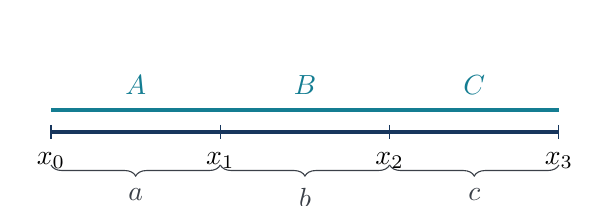
\begin{tikzpicture}[x=2.15cm,y=1cm,>=Latex]
  \draw[very thick,navy] (0,0)--(3,0);
  \foreach \x/\lab in {0/{x_0},1/{x_1},2/{x_2},3/{x_3}}{
    \draw[navy] (\x,0.09)--(\x,-0.09);
    \node[below=4pt] at (\x,0) {$\lab$};
  }
  \draw[very thick,teal] (0,0.28)--(1,0.28);
  \draw[very thick,teal] (1,0.28)--(2,0.28);
  \draw[very thick,teal] (2,0.28)--(3,0.28);
  \node[above=2pt,teal] at (0.5,0.28) {$A$};
  \node[above=2pt,teal] at (1.5,0.28) {$B$};
  \node[above=2pt,teal] at (2.5,0.28) {$C$};
  \draw[decorate,decoration={brace,amplitude=4pt,mirror},darkgray]
      (0,-0.42)--(1,-0.42) node[midway,below=5pt] {$a$};
  \draw[decorate,decoration={brace,amplitude=4pt,mirror},darkgray]
      (1,-0.42)--(2,-0.42) node[midway,below=5pt] {$b$};
  \draw[decorate,decoration={brace,amplitude=4pt,mirror},darkgray]
      (2,-0.42)--(3,-0.42) node[midway,below=5pt] {$c$};
\end{tikzpicture}
\end{center}

In a finite-dimensional tripartite system, conditional mutual information is
\begin{equation}\label{eq:finite-cmi}
 I(A:C\mid B)
 =S(AB)+S(BC)-S(B)-S(ABC)\ge 0.
\end{equation}
For a continuum CFT, however, each local algebra is type III and the individual von Neumann entropies in \eqref{eq:finite-cmi} are divergent.  Thus \eqref{eq:finite-cmi} may only be used as a mnemonic.  The finite object must be defined without subtracting four infinite numbers.

\section{The Longo--Xu input}

\subsection{Mutual information from Araki relative entropy}

Let \(U\) and \(V\) be separated regions.  Longo and Xu define the vacuum mutual information by
\begin{equation}\label{eq:MI-relative}
 \MI_{\cN}(U,V)
 :=\RE\!\left(\omega_{U\cup V}\,\middle\|\,
                 \omega_U\otimes_2\omega_V\right),
\end{equation}
where \(\RE(\cdot\|\cdot)\) is Araki relative entropy and \(\otimes_2\) is the graded product in the fermionic setting.  For a local even subnet it is the ordinary product state.

Throughout, \(\Ar\) denotes the net of \(r\) complex (Dirac) chiral fermions, \(\mathrm{CAR}(L^2(\mathbb R,\mathbb C^r))\), whose central charge is \(c=r\); Longo--Xu's Theorem~3.18 is stated for this net.  For \(\Ar\), Theorem~3.18 of Longo--Xu computes \eqref{eq:MI-relative} explicitly and, in particular, proves that it is finite.  If \(\cB\subset\Ar\) is a graded subnet, monotonicity of relative entropy gives
\begin{equation}\label{eq:subnet-bound}
 0\le \MI_{\cB}(U,V)\le \MI_{\Ar}(U,V)<\infty
\end{equation}
for separated \(U,V\) and every M\"obius covariant subnet \(\cB\subset\Ar\); this is shown in the proof of Theorem~4.1(6).

\subsection{Generalized mutual information is conditional mutual information}

For three pairwise separated regions \(X,Y,Z\), Longo and Xu introduce
\begin{equation}\label{eq:generalized-F}
\begin{split}
 \MI(X\cup Y,X\cup Z)
 :=\;&\MI(X,Y\cup Z)+\MI(Y,Z)\\
    &-\MI(X,Z)-\MI(X,Y).
\end{split}
\end{equation}
Their Theorem~4.1 proves, among other things, that this quantity is nonnegative and continuous from inside.  (Longo--Xu state the finite-dimensional limit formula below for pairwise separated \(X,Y,Z\); for the adjacent configuration used here it is combined with their equations (13)--(14), which define \(F\) for touching regions by the singular limit from inside.)  More importantly for the present question, their proof gives finite-dimensional factors \(X_n,Y_n,Z_n\) for which
\begin{equation}\label{eq:finite-approx}
\begin{split}
 \MI(X\cup Y,X\cup Z)
 =\lim_{n\to\infty}\big[&S(X_nY_n)+S(X_nZ_n)\\
                         &-S(X_n)-S(X_nY_nZ_n)\big].
\end{split}
\end{equation}
The bracket in \eqref{eq:finite-approx} is precisely the finite-dimensional conditional mutual information \(I(Y_n:Z_n\mid X_n)\).  Therefore the natural algebraic definition is
\begin{equation}\label{eq:cmi-as-F}
 \CMI(Y:Z\mid X):=\MI_{\cN}(X\cup Y,X\cup Z).
\end{equation}
Setting \(X=B\), \(Y=A\), and \(Z=C\) gives
\begin{equation}\label{eq:our-cmi}
 \CMI(A:C\mid B)=\MI_{\cN}(AB,BC)\ge 0.
\end{equation}
This explains why the generalized mutual information of the two overlapping intervals \(AB\) and \(BC\) is the correct continuum replacement for \eqref{eq:finite-cmi}.

\subsection{The finite-index singular-limit theorem}

For a finite-index subnet \(\cB\subset\Ar\), Theorem~4.2 supplies a regularized entropy functional \(G_{\cB}\) satisfying
\begin{equation}\label{eq:G-identity}
 \MI_{\cB}(U,V)
 =G_{\cB}(U)+G_{\cB}(V)-G_{\cB}(U\cup V)-G_{\cB}(U\cap V)
\end{equation}
for the extended, possibly overlapping, regions obtained by the Longo--Xu singular-limit prescription.  On a connected interval,
\begin{equation}\label{eq:G-connected}
 G_{\cB}((u,v))=\frac{r}{6}\log(v-u).
\end{equation}
The same formulas hold for \(\Ar\), and the paper explains how the construction passes to the finite-index extensions considered there.  Theorem~4.2 of Longo--Xu is stated for strongly additive nets (through their Theorem~4.4); \(\Ar\) and the finite-index extensions considered here are strongly additive.

The singular-limit condition is essential.  When a gap of size \(\eps\) closes, a universal divergent term \(P(\eps)\) appears in \(G\).  Since the same \(P(\eps)\) occurs with opposite signs in the balanced combination \eqref{eq:G-identity}, it cancels.  The next section makes this cancellation explicit.

\section{Proof of finiteness for three adjacent intervals}

\subsection{Direct proof from the \texorpdfstring{$G$}{G}-identity}

Apply \eqref{eq:G-identity} to the overlapping intervals \(AB=(x_0,x_2)\) and \(BC=(x_1,x_3)\).  Their union and intersection are
\[
 AB\cup BC=ABC=(x_0,x_3),\qquad AB\cap BC=B=(x_1,x_2).
\]
Hence, by \eqref{eq:G-connected},
\begin{align*}
 \CMI(A:C\mid B)
 &=G(AB)+G(BC)-G(ABC)-G(B)\\
 &=\frac{r}{6}\big[
      \log(x_2-x_0)+\log(x_3-x_1)\\
 &\hspace{4.5em}-\log(x_3-x_0)-\log(x_2-x_1)
    \big]\\
 &=\frac{r}{6}\log\!\left(
      \frac{(x_2-x_0)(x_3-x_1)}
           {(x_2-x_1)(x_3-x_0)}
    \right).
\end{align*}
All four lengths are finite and strictly positive, so the right-hand side is finite.  In terms of \(a,b,c\),
\begin{equation}\label{eq:abc-formula}
 \CMI(A:C\mid B)
 =\frac{r}{6}\log\!\left(
     \frac{(a+b)(b+c)}{b(a+b+c)}
   \right).
\end{equation}

\subsection{Gap regularization and cancellation of ultraviolet terms}

The same conclusion can be seen directly from the near-touching asymptotics in Theorem~4.2(2).  Introduce
\[
 A_{\eps}:=(x_0,x_1-\eps),\qquad
 D_d:=(x_1,x_1+d),\qquad \eps>0.
\]
Thus \(D_b=B\) and \(D_{b+c}=BC\), while \(A_{\eps}\) is separated from each by a gap \(\eps\).  Define the regulated chain-rule difference
\begin{equation}\label{eq:Ieps}
 I_{\eps}:=\MI(A_{\eps},D_{b+c})-\MI(A_{\eps},D_b).
\end{equation}
For every fixed \(\eps>0\), both terms are finite relative entropies.  Theorem~4.2(2) gives, for fixed \(d>0\),
\begin{equation}\label{eq:asymptotic}
 \MI(A_{\eps},D_d)
 =\frac{r}{6}\log\!\left(\frac{ad}{(a+d)\eps}\right)
  -\frac{1}{2}\log\mu_{\cN}+o(1),
 \qquad \eps\downarrow0,
\end{equation}
where \(\mu_{\cN}\) is the global index; for the free fermion net \(\mu_{\Ar}=1\).

Substitute \(d=b+c\) and \(d=b\) into \eqref{eq:asymptotic} and subtract.  The following terms cancel exactly:
\[
 -\frac{r}{6}\log\eps,\qquad
 \frac{r}{6}\log a,\qquad
 -\frac12\log\mu_{\cN}.
\]
Consequently,
\begin{align*}
 I_{\eps}
 &=\frac{r}{6}\left[
      \log\frac{b+c}{a+b+c}
      -\log\frac{b}{a+b}
    \right]+o(1)\\
 &=\frac{r}{6}\log\!\left(
      \frac{(a+b)(b+c)}{b(a+b+c)}
    \right)+o(1).
\end{align*}
Taking \(\eps\downarrow0\) reproduces \eqref{eq:abc-formula}; the identification of the limit with \(F(AB,BC)\) uses Longo--Xu, Theorem~4.1(5) (continuity from inside) and the definition of \(F\) for touching regions.  This calculation shows explicitly why neither the ultraviolet divergence nor the finite-index constant survives in conditional mutual information.

\section{Positivity, cross ratio, and limiting checks}

Define
\begin{equation}\label{eq:eta}
 \eta:=\frac{b(a+b+c)}{(a+b)(b+c)}.
\end{equation}
Since
\[
 (a+b)(b+c)-b(a+b+c)=ac>0,
\]
we have \(0<\eta<1\).  Equation \eqref{eq:abc-formula} therefore becomes
\begin{equation}\label{eq:cross-ratio-final}
 \CMI(A:C\mid B)=-\frac{r}{6}\log\eta>0.
\end{equation}
This agrees with the nonnegativity obtained abstractly from strong subadditivity in \eqref{eq:finite-approx}.

Several limiting checks are immediate:
\begin{itemize}
  \item If \(a\downarrow0\) or \(c\downarrow0\), then \(\eta\uparrow1\) and the conditional mutual information tends to zero.
  \item If the conditioning interval becomes long, \(b\to\infty\), then
  \[
    \CMI(A:C\mid B)
    =\frac{r}{6}\frac{ac}{b^2}+O(b^{-3}),
  \]
  so correlations between the two exterior intervals are screened by the large middle interval.
  \item If \(b\downarrow0\), the expression diverges logarithmically.  Thus the theorem asserts finiteness for three intervals of strictly positive length, not uniform boundedness as the conditioning interval collapses.
\end{itemize}

\begin{scopebox}
The rigorous conclusion drawn directly from Longo and Xu is for the free chiral fermion net \(\Ar\), its finite-index subnets, and the finite-index extensions treated after their Theorem~4.2.  Their Remark~4.3 conjectures an analogous statement for arbitrary rational conformal nets, with \(r\) replaced by the central charge.  That broader claim is not needed for, and is not proved by, the argument above.  Likewise, a general full two-dimensional CFT requires an additional left--right analysis beyond the chiral theorem.
\end{scopebox}

\section{Conclusion}

The key observation is that the continuum CMI is not defined by separately evaluating four divergent local entropies.  Longo and Xu's generalized mutual information provides the finite algebraic object
\[
 \CMI(A:C\mid B)=\MI(AB,BC).
\]
Theorem~4.1 identifies it as the limit of ordinary finite-dimensional conditional mutual informations and hence proves nonnegativity.  Theorem~4.2 controls the endpoint singularities in the finite-index class: the gap divergence and the global-index constant cancel in the conditional combination.  The remaining cutoff-independent quantity is the finite cross-ratio expression \eqref{eq:cross-ratio-final}.

\begin{thebibliography}{9}
\bibitem{LongoXu2018}
R.~Longo and F.~Xu,
\emph{Relative entropy in CFT},
Advances in Mathematics \textbf{337} (2018), 139--170.
\href{https://doi.org/10.1016/j.aim.2018.08.015}{doi:10.1016/j.aim.2018.08.015};
\href{https://arxiv.org/abs/1712.07283}{arXiv:1712.07283}.
\end{thebibliography}

\end{document}
